\documentclass{article}
\usepackage[utf8]{inputenc}
\usepackage{graphicx}
\usepackage[dvipsnames]{xcolor}
\usepackage{xcolor}
\usepackage{sectsty}
\usepackage{xcolor,colortbl}
\usepackage{float}
\usepackage{soul}
\usepackage{tikz}
\usepackage[english]{babel}
\usetikzlibrary{positioning}
 
\title{ECON 4P05 \\ Assignment 2: Classification Methods}
\author{ \\
Sannan Saleem 5889431}


\begin{document}
%color
\sectionfont{\color{PineGreen}}
\subsectionfont{\color{Maroon}}
\subsubsectionfont{\color{MidnightBlue}}

\maketitle

%outer border
\begin{tikzpicture}[remember picture,overlay]
     \draw[Yellow!70!black,line width=4pt] 
     ([xshift=-1.5cm,yshift=-2cm]current page.north east) coordinate (A)--([xshift=1.5cm,yshift=-2cm]current page.north west) coordinate(B)--([xshift=1.5cm,yshift=2cm]current page.south west) coordinate (C)--([xshift=-1.5cm,yshift=2cm]current page.south east) coordinate(D)--cycle;
\end{tikzpicture}

%inner border

\begin{tikzpicture}[remember picture,overlay]
     \draw[PineGreen!40!WildStrawberry,line width=4.5pt] 
     ([xshift=-2cm,yshift=-2.5cm]current page.north east) coordinate (A)--([xshift=2cm,yshift=-2.5cm]current page.north west) coordinate(B)--([xshift=2cm,yshift=2.5cm]current page.south west) coordinate (C)--([xshift=-2cm,yshift=2.5cm]current page.south east) coordinate(D)--cycle;
\end{tikzpicture}

\newpage
\tableofcontents
\newpage
\listoftables




\newpage
\section{Introduction}

In this assignment, we will be analyzing the Caravan data set through logistic regression, the linear probability model, the linear discriminant analysis and KNN.


\section{Classification methods}

\subsection{Describing the data set}

The Caravan data set uses 5822 real customer records and is owned and supplied by the Dutch data-mining company, Sentient Machine Research, and is based on real world business data. Within this data set are 86 variables that contain socio-demographic data derived from zip area codes (variables 1-43) and product ownership and usage (variables 44-86). The final variable, variable 86, pertains to if a customer had purchased a caravan insurance policy, which is especially important in this assignment as we are attempting to predict who would be interested in buying a caravan insurance policy with different models.  A classification problem requires that examples be classified into one of two or more classes. In this data set, we can classify each individual into one of two classes; purchased insurance or did not purchase insurance. A classification can have real-valued or discrete input variables, where in this case, we are using discrete input variables; 0 for not purchased and 1 for purchased. A problem with two classes is often called a two-class or binary classification problem.

\subsection{Fractions and error rates}
The fraction of people who purchased insurance is 348 (number of people who purchased insurance) /5822 (  number of people), yielding a   of 0.05977 or 5.98\%. To do this, we created a data frame from the ISLR and Caravan packages to present the 5822 observations and 86 variables.Using this dataframe, we created a table using the table function. By taking the purchase variable and appending it to the dataframe, and used the "ifany" command to compute the fraction of people who purchased insurance, as it take the number of people who were classified as "yes" and divides by the   number of people. The function "prop.table" which expresses table entries as a fraction of the marginal table, then rounded to 2 decimal places and multiplied by 100 to get a percentage. If we always predicted that someone would not buy insurance, the error rate would be the number of the people who actually bought insurance were the people who "deviated" from this. Therefore the number of people who bought insurance (348) divided by the   number of people in the data frame (5822) would result in the error rate of 0.05977 or 5.98\%. This was computed in R studio the same way as finding the fraction of people who purchased insurance.

\subsection{Two LPM Regressions}
The standard error of the regression for our model with a constant yielded 0.2371, while the model with all 85 predictors yielded 0.2283. Since the SER represents the average distance that the observed values fall from the regression line, the model with the smaller value is better because it indicates that the observations are closer to the fitted line. In this case, the the model with all 85 predictors is better than the model with a constant. \\
The value of the AIC for the full regression was calculated to be -505.1366. \\
9 coefficients were calculated to be statistically significant at a significance level of 6\%  and 23 coefficients were calculated to be significant at a significance level of 17\%.

\subsection{Computing the predicted probabilities}
By computing the predicted probabilities, we find the following features:\\
$$ min=-0.17130$$ $$max= 0.83797$$ $$mean=0.05977 $$\\
\newline
For an LPM probability to be sensible, it must be between the values of 0 and 1. When analyzing the predicted probabilities, the minimum probability is not sensible as it is a negative number, therefore not between 0 and 1, and not a well predicted probability. As a result of both the maximum and mean probabilities being between 0 and 1, we can conclude that the two LPM probabilities are sensible.\\
\newline
Upon examining the confusion matrix, we find the fraction of individuals that are correctly predicted to buy insurance (i.e. positive predicted value), as given by the confusionMatrix() command, is reported to be 0.9956 or 99.56\%.

\newline
Overall fraction of incorrect prediction is computed by:
$$ Overall incorrect predictions =  \frac{(False positive + False negative)}{(False positive + False negative + True positive + True negative)}  $$
therefore 
$$ Overall incorrect prediction = \frac{(24 + 333)}{24+333+15+5450} $$
yielding an overall incorrect prediction value of 0.0675 or 6.75\%. \\


Based on the results of the confusion matrix, we can see that we are really not conservative to consider the results as not purchasing insurance, and as such we predict most individuals do not buy insurance. Of course, this means that we find a really high percentage of the true negatives, but with a big trade off, and that is that we find also 333 False negatives. The is a low number of true positives compared to true negatives meaning that this model may not be the best to predict which people would buy insurance.\\
\newline

\begin{table}[!htb]
\caption{LPM confusion matrix}
\label{model1}
\begin{center}

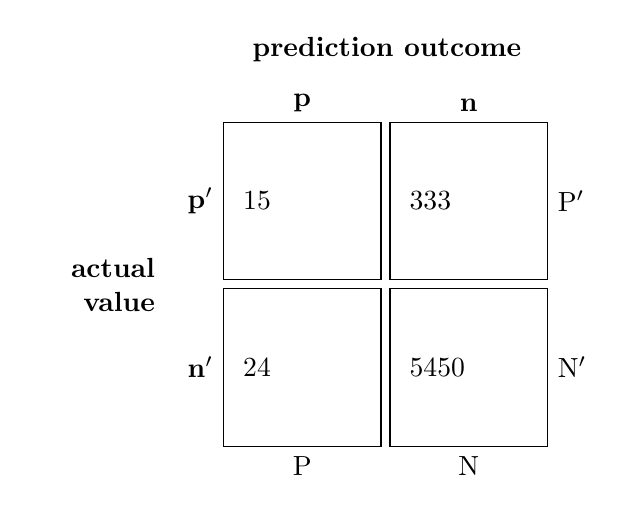
\begin{tikzpicture}[
box/.style={draw,rectangle,minimum size=2cm,text width=1.5cm,align=left}]
\matrix (conmat) [row sep=.1cm,column sep=.1cm] {
\node (tpos) [box,
    label=left:\( \mathbf{p'} \),
    label=above:\( \mathbf{p} \),
    ] {15};
&
\node (fneg) [box,
    label=above:\textbf{n},
    label=above right:\textbf{},
    label=right:\( \mathrm{P}' \)] {333};
\\
\node (fpos) [box,
    label=left:\( \mathbf{n'} \),
    label=below left:\textbf{},
    label=below:P] {24};
&
\node (tneg) [box,
    label=right:\( \mathrm{N}' \),
    label=below:N] {5450};
\\
};
\node [left=.05cm of conmat,text width=1.5cm,align=right] {\textbf{actual \\ value}};
\node [above=.05cm of conmat] {\textbf{prediction outcome}};
\end{tikzpicture}

\end{center}
\end{table}





\subsection{Selling insurance at random}

If the insurance company tries to sell insurance at random, the best success rate they can have is 6\%. In our data set of 5822 people, the highest amount of people the insurance company can sell to is (6/100) x 5288 = 317 people. This could be very costly especially if the broker needs to visit everyone he/she tries to sell insurance to as it would take a lot more time, more labor, and hence, as previously mentioned, be more costly. By analyzing our linear probability model with all variables, we can compute the confusion matrix and find the fraction of individuals that are correctly predicted to buy insurance (i.e. positive predicted value) to be 0.9979 or 99.79\%. This 99.79\% positive predicted value of people who were predicted to buy insurance and actually did is much higher than the insurance company trying to sell insurance at random and receiving a 6\% success rate. Through the LPM we know that if the insurance company were to only sell to customers who are likely to buy, they could increase their success rate from 6\% when the were randomly selling, all the way to 99.79\% by targeting the people who are predicted to buy insurance, as per the LPM model. 



\subsection{logistic regression}

\begin{table}[!htb]
\caption{Logistic regression confusion matrix with cut off at 0.5}
\label{model1}
\begin{center}

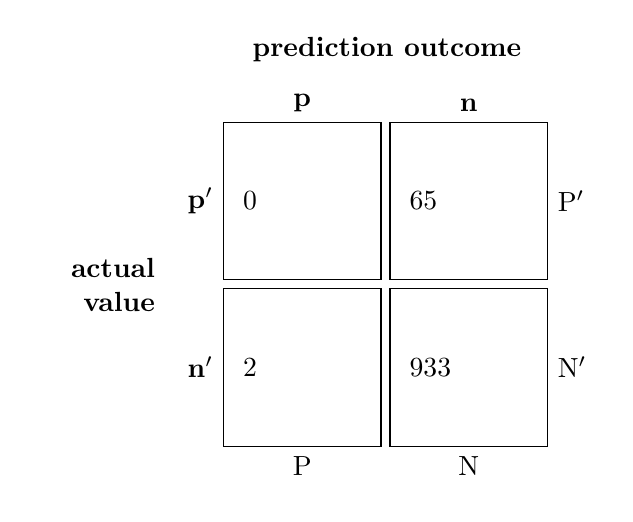
\begin{tikzpicture}[
box/.style={draw,rectangle,minimum size=2cm,text width=1.5cm,align=left}]
\matrix (conmat) [row sep=.1cm,column sep=.1cm] {
\node (tpos) [box,
    label=left:\( \mathbf{p'} \),
    label=above:\( \mathbf{p} \),
    ] {0};
&
\node (fneg) [box,
    label=above:\textbf{n},
    label=above right:\textbf{},
    label=right:\( \mathrm{P}' \)] {65};
\\
\node (fpos) [box,
    label=left:\( \mathbf{n'} \),
    label=below left:\textbf{},
    label=below:P] {2};
&
\node (tneg) [box,
    label=right:\( \mathrm{N}' \),
    label=below:N] {933};
\\
};
\node [left=.05cm of conmat,text width=1.5cm,align=right] {\textbf{actual \\ value}};
\node [above=.05cm of conmat] {\textbf{prediction outcome}};
\end{tikzpicture}

\end{center}
\end{table}

The fraction of individuals that are correctly predicted to buy insurance in the logistic regression using a cut-off of 0.5 (i.e. the positive predicted value) was computed to be 0.9979 or 99.79\%. 

\newline

\begin{table}[!htb]
\caption{Logistic regression confusion matrix with cut off at 0.25}
\label{model1}
\begin{center}

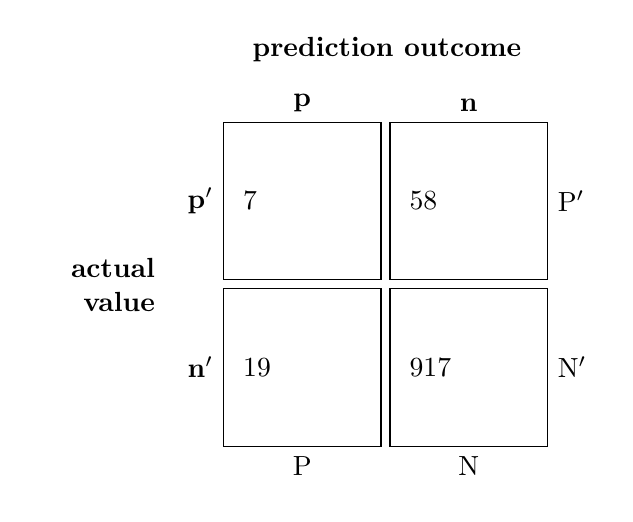
\begin{tikzpicture}[
box/.style={draw,rectangle,minimum size=2cm,text width=1.5cm,align=left}]
\matrix (conmat) [row sep=.1cm,column sep=.1cm] {
\node (tpos) [box,
    label=left:\( \mathbf{p'} \),
    label=above:\( \mathbf{p} \),
    ] {7};
&
\node (fneg) [box,
    label=above:\textbf{n},
    label=above right:\textbf{ },
    label=right:\( \mathrm{P}' \)] {58};
\\
\node (fpos) [box,
    label=left:\( \mathbf{n'} \),
    label=below left:\textbf{ },
    label=below:P] {19};
&
\node (tneg) [box,
    label=right:\( \mathrm{N}' \),
    label=below:N] {917};
\\
};
\node [left=.05cm of conmat,text width=1.5cm,align=right] {\textbf{actual \\ value}};
\node [above=.05cm of conmat] {\textbf{prediction outcome}};
\end{tikzpicture}

\end{center}
\end{table}

The fraction of individuals that are correctly predicted to buy insurance in the logistic regression using a cut-off of 0.25 (i.e. the positive predicted value) was computed to be 0.9807 or 9.09\%. 
\newline
Comparing this to the random guessing success rate of 6\%, we can conclude that the logistic model at is better as it yields more people being correctly predicted to buy insurance than the random guessing.\\
\newline

\subsection{KNN with K=1,2,3}

\begin{table}[!htb]
\caption{KNN with K=1}
\label{model1}
\begin{center}

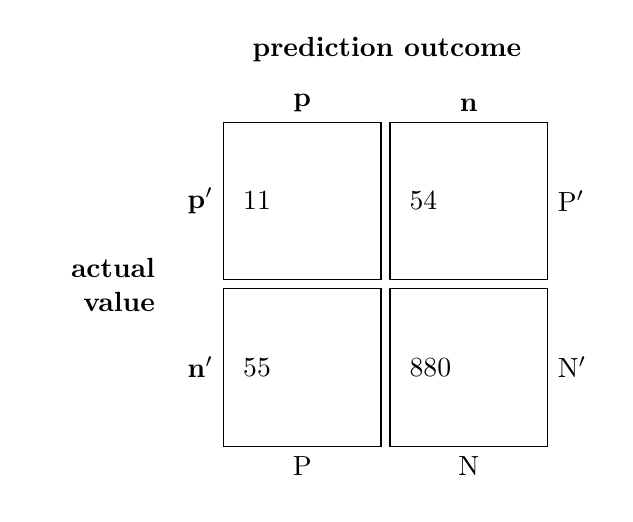
\begin{tikzpicture}[
box/.style={draw,rectangle,minimum size=2cm,text width=1.5cm,align=left}]
\matrix (conmat) [row sep=.1cm,column sep=.1cm] {
\node (tpos) [box,
    label=left:\( \mathbf{p'} \),
    label=above:\( \mathbf{p} \),
    ] {11};
&
\node (fneg) [box,
    label=above:\textbf{n},
    label=above right:\textbf{ },
    label=right:\( \mathrm{P}' \)] {54};
\\
\node (fpos) [box,
    label=left:\( \mathbf{n'} \),
    label=below left:\textbf{},
    label=below:P] {55};
&
\node (tneg) [box,
    label=right:\( \mathrm{N}' \),
    label=below:N] {880};
\\
};
\node [left=.05cm of conmat,text width=1.5cm,align=right] {\textbf{actual \\ value}};
\node [above=.05cm of conmat] {\textbf{prediction outcome}};
\end{tikzpicture}



\end{center}
\end{table}

 
 

By computing the confusion matrix of the KNN model with k=1, we find the Positive Predictive Value to be 0.9412, therefore the percentage of individuals that are correctly predicted to buy insurance is 94.12\% in this data set. Comparing this to the random guessing success rate of 6\%, we can conclude that the KNN model at K=1 is better.\\
\newpage


\begin{table}[!htb]
\caption{KNN with K=3}
\label{model1}
\begin{center}

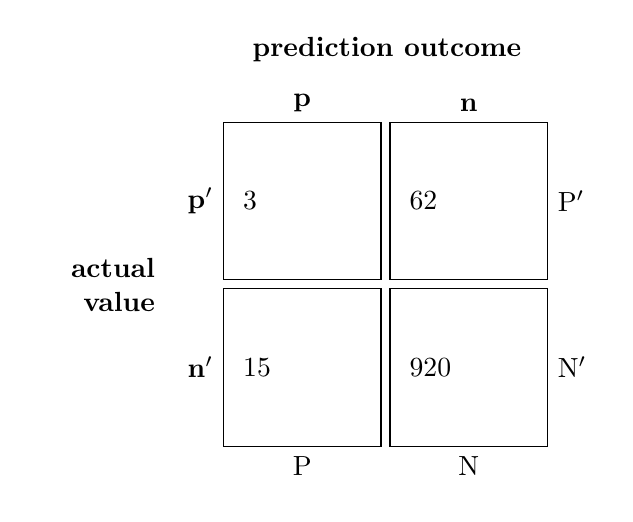
\begin{tikzpicture}[
box/.style={draw,rectangle,minimum size=2cm,text width=1.5cm,align=left}]
\matrix (conmat) [row sep=.1cm,column sep=.1cm] {
\node (tpos) [box,
    label=left:\( \mathbf{p'} \),
    label=above:\( \mathbf{p} \),
    ] {3};
&
\node (fneg) [box,
    label=above:\textbf{n},
    label=above right:\textbf{},
    label=right:\( \mathrm{P}' \)] {62};
\\
\node (fpos) [box,
    label=left:\( \mathbf{n'} \),
    label=below left:\textbf{},
    label=below:P] {15};
&
\node (tneg) [box,
    label=right:\( \mathrm{N}' \),
    label=below:N] {920};
\\
};
\node [left=.05cm of conmat,text width=1.5cm,align=right] {\textbf{actual \\ value}};
\node [above=.05cm of conmat] {\textbf{prediction outcome}};
\end{tikzpicture}

\end{center}
\end{table}

By computing the confusion matrix of the KNN model with k=3, we find the Positive Predictive Value to be 0.98396, therefore the percentage of individuals that are correctly predicted to buy insurance is 98.4\% in this data set. Comparing this to the random guessing success rate of 6\%, we can conclude that the KNN model at K=3 is better.\\

\newpage

\begin{table}[!htb]
\caption{KNN with K=5}
\label{model1}
\begin{center}

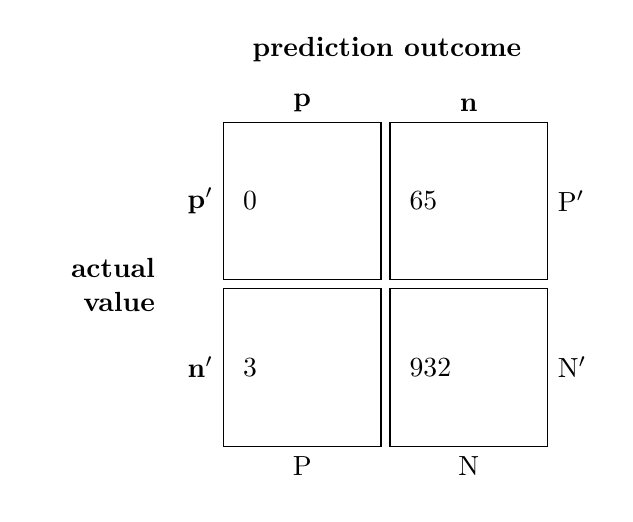
\begin{tikzpicture}[
box/.style={draw,rectangle,minimum size=2cm,text width=1.5cm,align=left}]
\matrix (conmat) [row sep=.1cm,column sep=.1cm] {
\node (tpos) [box,
    label=left:\( \mathbf{p'} \),
    label=above:\( \mathbf{p} \),
    ] {0};
&
\node (fneg) [box,
    label=above:\textbf{n},
    label=above right:\textbf{ },
    label=right:\( \mathrm{P}' \)] {65};
\\
\node (fpos) [box,
    label=left:\( \mathbf{n'} \),
    label=below left:\textbf{ },
    label=below:P] {3};
&
\node (tneg) [box,
    label=right:\( \mathrm{N}' \),
    label=below:N] {932};
\\
};
\node [left=.05cm of conmat,text width=1.5cm,align=right] {\textbf{actual \\ value}};
\node [above=.05cm of conmat] {\textbf{prediction outcome}};
\end{tikzpicture}

\end{center}
\end{table}





By computing the confusion matrix of the KNN model with k=5, we find the Positive Predictive Value to be 0.9968, therefore the percentage of individuals that are correctly predicted to buy insurance is 99.68\% in this data set. Comparing this to the random guessing success rate of 6\%, we can conclude that the KNN model at K=5 is better.\\
\newline

The final statement is that for all three K, the result is better than random guessing.
\newpage

\subsection{Confusion Matrix using LDA}

\begin{table}[!htb]
\caption{LDA confusion matrix}
\label{model1}
\begin{center}

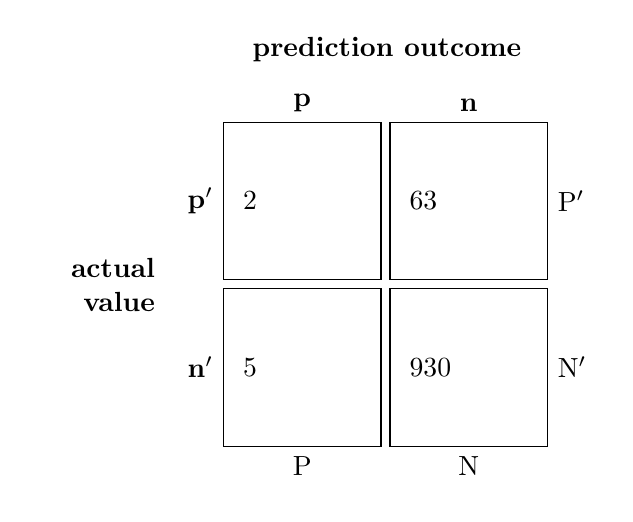
\begin{tikzpicture}[
box/.style={draw,rectangle,minimum size=2cm,text width=1.5cm,align=left}]
\matrix (conmat) [row sep=.1cm,column sep=.1cm] {
\node (tpos) [box,
    label=left:\( \mathbf{p'} \),
    label=above:\( \mathbf{p} \),
    ] {2};
&
\node (fneg) [box,
    label=above:\textbf{n},
    label=above right:\textbf{},
    label=right:\( \mathrm{P}' \)] {63};
\\
\node (fpos) [box,
    label=left:\( \mathbf{n'} \),
    label=below left:\textbf{},
    label=below:P] {5};
&
\node (tneg) [box,
    label=right:\( \mathrm{N}' \),
    label=below:N] {930};
\\
};
\node [left=.05cm of conmat,text width=1.5cm,align=right] {\textbf{actual \\ value}};
\node [above=.05cm of conmat] {\textbf{prediction outcome}};
\end{tikzpicture}

\end{center}
\end{table}


By computing the confusion matrix of the LDA model, we find the Positive Predictive Value to be 0.99465, therefore the percentage of individuals that are correctly predicted to buy insurance is 99.46\% in this data set. Comparing this to the random guessing success rate of 6\%, we can conclude that the LDA model is better.

\subsection{Which provides the best Results; Logistic, KNN or LDA}

When analyzing our results, we found that KNN appears to provide the best results on this data, specifically when K=5. This is because it provides the highest percentage of people who were predicted to buy insurance and actually did, compared to LDA and logistic which provided the lowest percentages. 

\section{Conclusion}
In conclusion, after testing the Caravan data set with a logistic model, linear probability model, linear discriminant analysis and KNN at different K's, it is clear to see that KNN provides the best results in testing individuals who were predicted to buy insurance and actually did, when computing the confusion matrix and analyzing positive predicted values of each confusion matrix.

\newpage

\section{Appendix}

\subsection{Work Cited}
James, G., Witten, D., Hastie, T., & Tibshirani, R. (2013). An Introduction to Statistical Learning: with Applications in R (Springer Texts in Statistics) (1st ed. 2013, Corr. 7th printing 2017 ed.) [E-book].\\
Springer. https://lms.brocku.ca/access/lessonbuilder/item/47651720/group/7e42f3bc-9d92-4e41-bf41-4ec95e1bd241/Lessons/ISLR%20Seventh%20Printing.pdf

\subsection{R Input}
\begin{verbatim}
install.packages("ISLR")
install.packages("tidyverse")
install.packages(c("caret", "class", "MASS", "rstatix", "psych", "e1071"))
install.packages("standardize")
library(MASS)
library(caret)
library(tidyverse)
library(ISLR)
library(standardize)



set.seed(12)



df <- ISLR::Caravan



#Q1
help("Caravan")
str(df)



# Q2
tb <- table(df$Purchase, useNA = "ifany")
round(prop.table(tb) * 100, 2)
#the fraction of people that purchased ins. is 348/5822~0.05977~5.98%



#assuming that everyone does not buy insurance the deviated i.e(ppl who did buy) would classify as the error =>
#error rate = 5.98% ((348/5822)*100)




# Create dummy var (called->dependent_var) 
df$dependent_var <- ifelse(df$Purchase == "Yes", 1, 0)



#drop purchase variable from dataframe
df$Purchase <- NULL




#Q3
#model with only constant
model_1 <- lm(formula = dependent_var ~  1, data = df)
summary(model_1)



#model with all vars
model_all <-lm(formula = dependent_var ~  ., data = df)
model_summary <- summary(model_all)
summary(model_all)



#calculate SER for maodel with 1 var
model_1 <- lm(formula = dependent_var ~ 1 , data = df)
summary(model_1)
model_1_summary <- summary(model_1)
model_1_summary
SSR <- sum(model_1_summary$residuals^2)
n <- nrow(Caravan)
SER <- sqrt(SSR / (n-2))



#calculate SER for maodel with all vars
model_all <-lm(formula = dependent_var ~  ., data = df)
model_summary <- summary(model_all)
model_summary
SSR_all <- sum(model_summary$residuals^2)
SER_all <- sqrt(SSR_all / (n-2))




#calculate aic and store it as aic_model
AIC(object = model_all)
aic_model <- AIC(object = model_all)



#Q4
#isolae p-value column 
prob <- coef(summary(model_all))[, "Pr(>|t|)"]



#create "loop" 
#significance at 6%
sign_6 <- ifelse(prob < 0.06, 1, 0)
table(sign_6)



#significance at 17%
sign_17 <- ifelse(prob < 0.17, 1, 0)
table(sign_17)



# compute predicted probabilities
predicted_value <- predict(object = model_all, newdata = df)



predicted_value
#gain insight on min/max/mean
summary(predicted_value)
#min=-0.17130 max=0.83787 mean=0.05396



#create confusion matrix
predicted_value <- ifelse(predicted_value > 0.3, 1, 0)
table(predicted_value)
LPM_contb <- table(df$dependent_var, predicted_value,  deparse.level = 2)
confusionMatrix(LPM_contb)


# Q5
Selected <- sample.int(nrow(df), 1000)
# index selected the row; use [col,row] pattern to select rows
x_test <- df[ Selected, ] 
# use -index to remove rows
x_train  <- df[-Selected, ] 



xTest_scaled <- x_test
xTrain_scaled<- x_train
xTest_scaled[c(1:85)] <- lapply(xTest_scaled[c(1:85)], function(x) c(scale(x)))
xTrain_scaled[c(1:85)] <- lapply(xTrain_scaled[c(1:85)], function(x) c(scale(x)))
xTest_scaled$AZEILPL <- NULL
xTest_scaled$PZEILPL <- NULL
xTrain_scaled$AZEILPL <- NULL
xTrain_scaled$PZEILPL <- NULL



#Q6
# create Logistic regression w/ cut-off @ 0.5
model_logistic <- glm(formula = dependent_var ~  ., data = x_train, family = "binomial"(link = "logit"))
summary(model_logistic)
predicted_value_log_5 <- predict(object = model_logistic, newdata = x_test ,type="response")
#confusion matrix w/ cut-off @ 0.5
predicted_value_log_5 <- ifelse(predicted_value_log_5 > 0.5, 1, 0)
Log_conmx5 <- table(x_test$dependent_var, predicted_value_log_5, deparse.level = 2)
confusionMatrix(Log_conmx5)



# create Logistic regression w/ cut-off @ 0.25
model_logistic <- glm(formula = dependent_var ~  ., data = x_train, family = "binomial"(link = "logit"))
summary(model_logistic)
predicted_value_log_25 <- predict(object = model_logistic, newdata = x_test ,type="response")
#confusion matrix w/ cut-off @ 0.5
predicted_value_log_25 <- ifelse(predicted_value_log_25 > 0.25, 1, 0)
Log_conmx25 <- table(x_test$dependent_var, predicted_value_log_25, deparse.level = 2)
confusionMatrix(Log_conmx25)




#Q7
# Appliying KNN
knn_model_k1 <- class::knn(xTrain_scaled, xTest_scaled, xTrain_scaled$dependent_var, k = 1)
KNN_conmx_k1 <- table(x_test$dependent_var, knn_model_k1, deparse.level = 2)
confusionMatrix(KNN_conmx_k1)


knn_model_k3 <- class::knn(xTrain_scaled, xTest_scaled, x_train$dependent_var, k = 3)
KNN_conmx_k3 <- table(x_test$dependent_var, knn_model_k3, deparse.level = 2)
confusionMatrix(KNN_conmx_k3)



knn_model_k5 <- class::knn(xTrain_scaled, xTest_scaled, x_train$dependent_var, k = 5)
KNN_conmx_k5 <- table(x_test$dependent_var, knn_model_k5, deparse.level = 2)
confusionMatrix(KNN_conmx_k5)



#Q8
# Applying LDA
lda_model <- lda(dependent_var ~ ., data = x_train)
lda_predict <- predict(lda_model, x_test)
LDA_conmx <- table(x_test$dependent_var, lda_predict$class)
confusionMatrix(LDA_conmx)
\end{verbatim}

\end{document}